\documentclass{standalone}
\usepackage{tikz}
\usetikzlibrary{automata, positioning, arrows}

\begin{document}
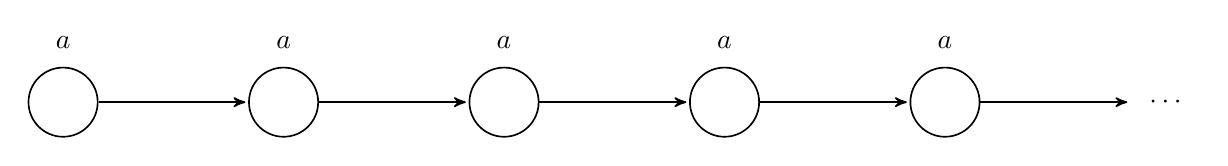
\begin{tikzpicture}[->,>=stealth',shorten >=1pt,auto,node distance=2.8cm,
                    semithick]
  \tikzstyle{every state}=[fill=white,draw=black,text=black]

  \node[state] (A)                    {};
  \node[state] (B) [right of=A]       {};
  \node[state] (C) [right of=B]       {};
  \node[state] (D) [right of=C]       {};
  \node[state] (E) [right of=D]       {};
  \node[state,draw=none] (F) [right of=E]       {$\cdots$};

  % Labels above nodes
  \node[above=0.1cm of A] {$a$};
  \node[above=0.1cm of B] {$a$};
  \node[above=0.1cm of C] {$a$};
  \node[above=0.1cm of D] {$a$};
  \node[above=0.1cm of E] {$a$};

  \path (A) edge              node {} (B)
        (B) edge              node {} (C)
        (C) edge              node {} (D)
        (D) edge              node {} (E)
        (E) edge              node {} (F);
\end{tikzpicture}
\end{document}